\documentclass[DIV=13, 10pt,a4paper]{scrartcl} %% Remove demo in your file.


\usepackage[utf8]{inputenc}
\usepackage[ngerman]{babel}
\usepackage{eurosym}
\usepackage{geometry}
\usepackage{xcolor,colortbl}
\usepackage{graphicx}
\usepackage[headsepline,footsepline,automark]{scrpage2}
\usepackage{pdfpages}
\usepackage{tabularx}
\usepackage{multicol}
\usepackage{multirow}
\usepackage{amssymb}
\usepackage{amsmath}

\usepackage{lipsum}% Used for dummy text.


\definecolor{titlepagecolor}{cmyk}{1,.60,0,.40}
\definecolor{namecolor}{cmyk}{0,.24,.07,.47} 

\makeatletter                       
\def\printauthor{%                  
	{\small \@author}}              
\makeatother
\author{%
	Author 1 name \\
	\texttt{email1@example.com}\vspace{10pt} \\
	Author 2 name \\
	\texttt{email2@example.com}\vspace{10pt} \\
	Author 3 name \\
	\texttt{email3@example.com}\vspace{10pt} \\
	Author 4 name \\
	\texttt{email4@example.com}
}


\pagestyle{scrheadings}
\cfoot[]{}
\ofoot[]{\pagemark}
\setkomafont{pageheadfoot}{\normalfont\sffamily}

\newcommand{\colorcell}[1]{\cellcolor{namecolor}\color{white}\textbf{#1}}
\newcommand{\colorcelllight}[1]{\cellcolor{namecolor!25}\color{black}{#1}}

%-----------------------------------------------------------------
\begin{document}
% ----------------------------------------------------------------
\begin{titlepage}

\newgeometry{left=3cm,right=4cm} %defines the geometry for the titlepage
\pagecolor{titlepagecolor}
\noindent

\includegraphics[width=3cm]{logo.jpg}\\[1em]
\color{white}
{\LARGE \textbf{\textsf{PPP - Pen\&Paper Pal}}}\\
\makebox[0pt][l]{\rule{1.3\textwidth}{1pt}}
\par
\noindent
\textbf{\textsf{Ostbayrische Technische Hochschule}} \textcolor{namecolor}{\textsf{Regensburg}}
\vfill
\noindent
\begin{minipage}[t]{0.35\linewidth}
	\vspace{0pt}
	\begin{flushright}
		\printauthor
	\end{flushright}
\end{minipage}
%\hspace{15pt}
\hfill
\begin{minipage}[t]{0.6\linewidth}
	\vspace{40pt}
	{\huge \textsf{Projektbericht}}
	\vskip\baselineskip
	\noindent
	\textsf{\today}
\end{minipage}
\end{titlepage}
\restoregeometry % restores the geometry
\nopagecolor% Use this to restore the color pages to white
% ----------------------------------------------------------------

\tableofcontents
\thispagestyle{empty}
\pagebreak
\setcounter{page}{1}

\section{Projektvision}
\thispagestyle{empty}
	\begin{flushleft}
		
\includegraphics[page=1,width=0.75\textwidth]{docs/presentation.pdf}
		\vfill
	\end{flushleft}
	\begin{center}
		
\includegraphics[page=2,width=0.75\textwidth]{docs/presentation.pdf}
		\vfill
	\end{center}
	\begin{flushright}
		
\includegraphics[page=3,width=0.75\textwidth]{docs/presentation.pdf}
	\end{flushright}
	

\section{Projektauftrag}
\begin{tabularx}{\textwidth}{|c|X|}
	\hline
	\colorcell{Projekttitel} & PPP - Pen\&Paper Pal\\
	\hline
\end{tabularx}
\newline
\vspace{2pt}
\newline
\begin{tabularx}{\textwidth}{|l|X|l|X|}
	\hline
	\multicolumn{4}{|l|}{\colorcell{Projektdaten}}\\
	\hline
	\colorcelllight{Start} & 28.03.2018 & \colorcelllight{Projektkategorie} & Kleinprojekt\\
	\cline{2-2} \cline{4-4}
	\colorcelllight{Ende} & 10.07.2018 & \colorcelllight{Projektnummer} & 420\\
	\hline
\end{tabularx}
\newline
\vspace{2pt}
\newline
\begin{tabularx}{\textwidth}{|l|X|l|X|}
	\hline
	\multicolumn{4}{|l|}{\colorcell{Projektorganisation}} \\
	\hline
	\colorcelllight{Projektmanager*in} & Markus Bauer & \colorcelllight{Projektauftraggeber*in} & Carsten Kern\\
	\cline{2-4}
	\colorcelllight{} &\multicolumn{1}{l}{Patrick Gruber}& \multicolumn{1}{l}{Richard Tscharntke}  & \\
	\multirow{-2}{*}{\colorcelllight{Projektteammitglieder}}& \multicolumn{1}{l}{Marius Tuschl} & \multicolumn{1}{l}{Markus Bauer}& \\
	\hline
\end{tabularx}
\newline
\vspace{2pt}
\newline
\begin{tabularx}{\textwidth}{|l|X|}
	\hline
	\multicolumn{2}{|l|}{\colorcell{Projektbeschreibung}}\\
	\hline
	\colorcelllight{Projektbegründung} & Es ist aufwendig Mitspieler für Gesellschaftsspiele zu finden.\\
	\cline{2-2}
	\colorcelllight{Projektgesamtziel} & Entwicklung und Deployment eines sozialen Netzwerkes zur Suche und Organisation von Mitspielern für Gesellschaftsspiele. Der Zugriff auf das Netzwerk erfolgt über eine mobile Applikation auf den aktuellen Android Versionen.\\
	\hline
	\multicolumn{1}{|l}{\colorcell{Projektteilziele $\Rightarrow$}} & \multicolumn{1}{l|}{\colorcell{Messbare Ergebnisse}}\\
	\hline
	Backend & Funktionalitäten können über API verwendet werden.\\
	\cline{2-2}
	Anmeldung & User können  einn Profil erstellen.\\
	\cline{2-2}
	Suche & User können andere User finden.\\
	\cline{2-2}
	Filter & User können nach Spiel, Ort, Datum, durchschnittlichem Alter und Geschlecht filtern.\\
	\cline{2-2}
	Bewertung & User können andere User und Spiele anhand verschiedener Kriterien bewerten.\\
	\cline{2-2}
	Gruppen & User können sich in Gruppen zusammenschließen, per Chat unterhalten und mit einem Kalender gemeinsame Termine verwalten.\\
	\cline{2-2}
	Tauschbörse & User können auf einer Tauschbörse Spiele im Tausch gegen andere Spiele suchen und anbieten. \\
	\cline{2-2}
	Forum & User können in einem für jeden User zugänglichen Forum Informationen austauschen.\\
	\cline{2-2}
	Werbeintegration & In unserer App kann über ADSense Werbung geschalten werden.\\
	\hline
	\colorcelllight{Nicht-Ziele} & Exklusion\\
	\cline{2-2}
	\colorcelllight{Wirkung/Nutzen} & Inklusion.\\
	\hline
	\colorcelllight{} & 1. Backend implementieren.\\
	\cline{2-2}
	\colorcelllight{} & 2. Fronntend implementieren.\\
	\cline{2-2}
	\colorcelllight{} & 3. Testen.\\
	\cline{2-2}
	\colorcelllight{} & 4. Dezentralisierten Coin Miner implementieren.\\
	\cline{2-2}
	\multirow{-5}{*}{\colorcelllight{Projektphasen}} & 5. Get rich fast! \\
	\hline
	\colorcelllight{} & Zu wenig User.\\
	\cline{2-2}
	\colorcelllight{} & Server nicht errichbar. Datenbanksicherheit.\\
	\cline{2-2}
	\colorcelllight{} & Zu viele User und dadurch resultierende lange Latenz am Server.\\
	\cline{2-2}
	\colorcelllight{} & Zu lange Zeit zwischen initialem und feature Release.\\
	\cline{2-2}
	\multirow{-5}{*}{\colorcelllight{Projektrisiken}} & Unintuitives UserInterface.\\
	\hline
\end{tabularx}
\newline
\vspace{2pt}
\newline
\begin{tabularx}{\textwidth}{|l|X|}
	\hline
	\multicolumn{2}{|l|}{\colorcell{Projektbudget \& Wirtschaftlichkeit}}\\
	\hline
	\colorcelllight{} & Beteiligter + Aufwand in STD oder Tagen.\\
	\cline{2-2}
	\colorcelllight{} & Beteiligter + Aufwand in STD oder Tagen.\\
	\cline{2-2}
	\colorcelllight{} & Beteiligter + Aufwand in STD oder Tagen.\\
	\cline{2-2}
	\multirow{-4}{*}{\colorcelllight{Personalkosten}} & Beteiligter + Aufwand in STD oder Tagen.\\
	\hline
	\colorcelllight{Summe Pers.Kosten} & Summe in \euro Personalaufwand mal ind.Stundensätze.\\
	\hline
	\colorcelllight{} &  zB Beratungskosten in \euro.\\
	\cline{2-2}
	\colorcelllight{} & Kostenposition in \euro.\\
	\cline{2-2}
	\multirow{-3}{*}{\colorcelllight{Ausgabewirksame Kosten}} & Kostenposition in \euro.\\
	\hline
	\colorcelllight{Sonstige Ressourcen} & zB Maschinen, Labore, Räume.\\
	\hline
	\colorcelllight{Projekbudget} & in \euro\\
	\hline
	\colorcelllight{Wirtschaftlichkeit} & Sind während oder nach Beendigung des Projekts Einnahmen zu erwarten, mit denen die Projektkosten kompensiert werden können?\\
	\hline
	\colorcelllight{Folgekosten} & Entstehen Folgekosten, die bereits jetzt berücksichtigt werden müssen?\\
	\hline
\end{tabularx}
\newline
\vspace{2pt}
\newline
\begin{tabularx}{\textwidth}{|l|X|X|X|X|}
	\hline
	\colorcell{Projektkategorisierung} &0 & 1 & 2 & 3\\
	\hline
	\colorcelllight{strategische Bedeutung} & & & &\\
	\cline{2-5}
	\colorcelllight{Risikogehalt} & & & & \\
	\cline{2-5}
	\colorcelllight{Komplexitätsgrad} & & & & \\
	\cline{2-5}
	\colorcelllight{Neuartigskeitsgrad} & & & & \\
	\cline{2-5}
	\colorcelllight{Termindurck} & & & & \\
	\cline{2-5}
	\colorcelllight{Klarheit über Projektziele} & & & & \\
	\hline
\end{tabularx}
\newline
\vspace{2pt}
\newline
\begin{tabularx}{\textwidth}{|l|X|}
	\hline
	\multicolumn{2}{|l|}{\colorcell{Sonstiges}}\\
	\hline
	Sonstige relevante Informationenn & \\
	\hline
\end{tabularx}
\newline
\vspace{2pt}
\newline
\begin{tabularx}{\textwidth}{|l|lXr|}
	\hline
	\colorcell{} & Projekt wird bewilligt& &$\square$ \\
	\cline{2-4}
	\colorcell{} & Projekt wird abgeleht & & $\square$ \\
	\cline{2-4}
	\colorcell{} & Begründung & & \\
	\colorcell{} & & & \\
	\colorcell{} & & & \\
	\cline{2-4}
	\colorcell{} & Datum & & \\
	\cline{2-4}
	\multirow{-6}{*}{\colorcell{Projektentscheidung}} & Auftraggeber*in & &\\
	\hline
\end{tabularx}

\newpage

\section{Umsetzbarkeit}
\begin{multicols}{2}
	\subsection*{Basissystem}
		\begin{itemize}
			\item User
			\item Adress
			\item Location
			\item Game
			\item Rating
			\item Group
			\item Advertisement
		\end{itemize}
	\subsection*{Chatsystem}
		\begin{itemize}
			\item Chat
			\item Message
		\end{itemize}
	\subsection*{Forumsystem}
		\begin{itemize}
			\item Forum
			\item Thread
			\item TradeThread
			\item Post
		\end{itemize}
\end{multicols}

\section{Systemkontext}
\begin{figure}[h!]
	\centering
	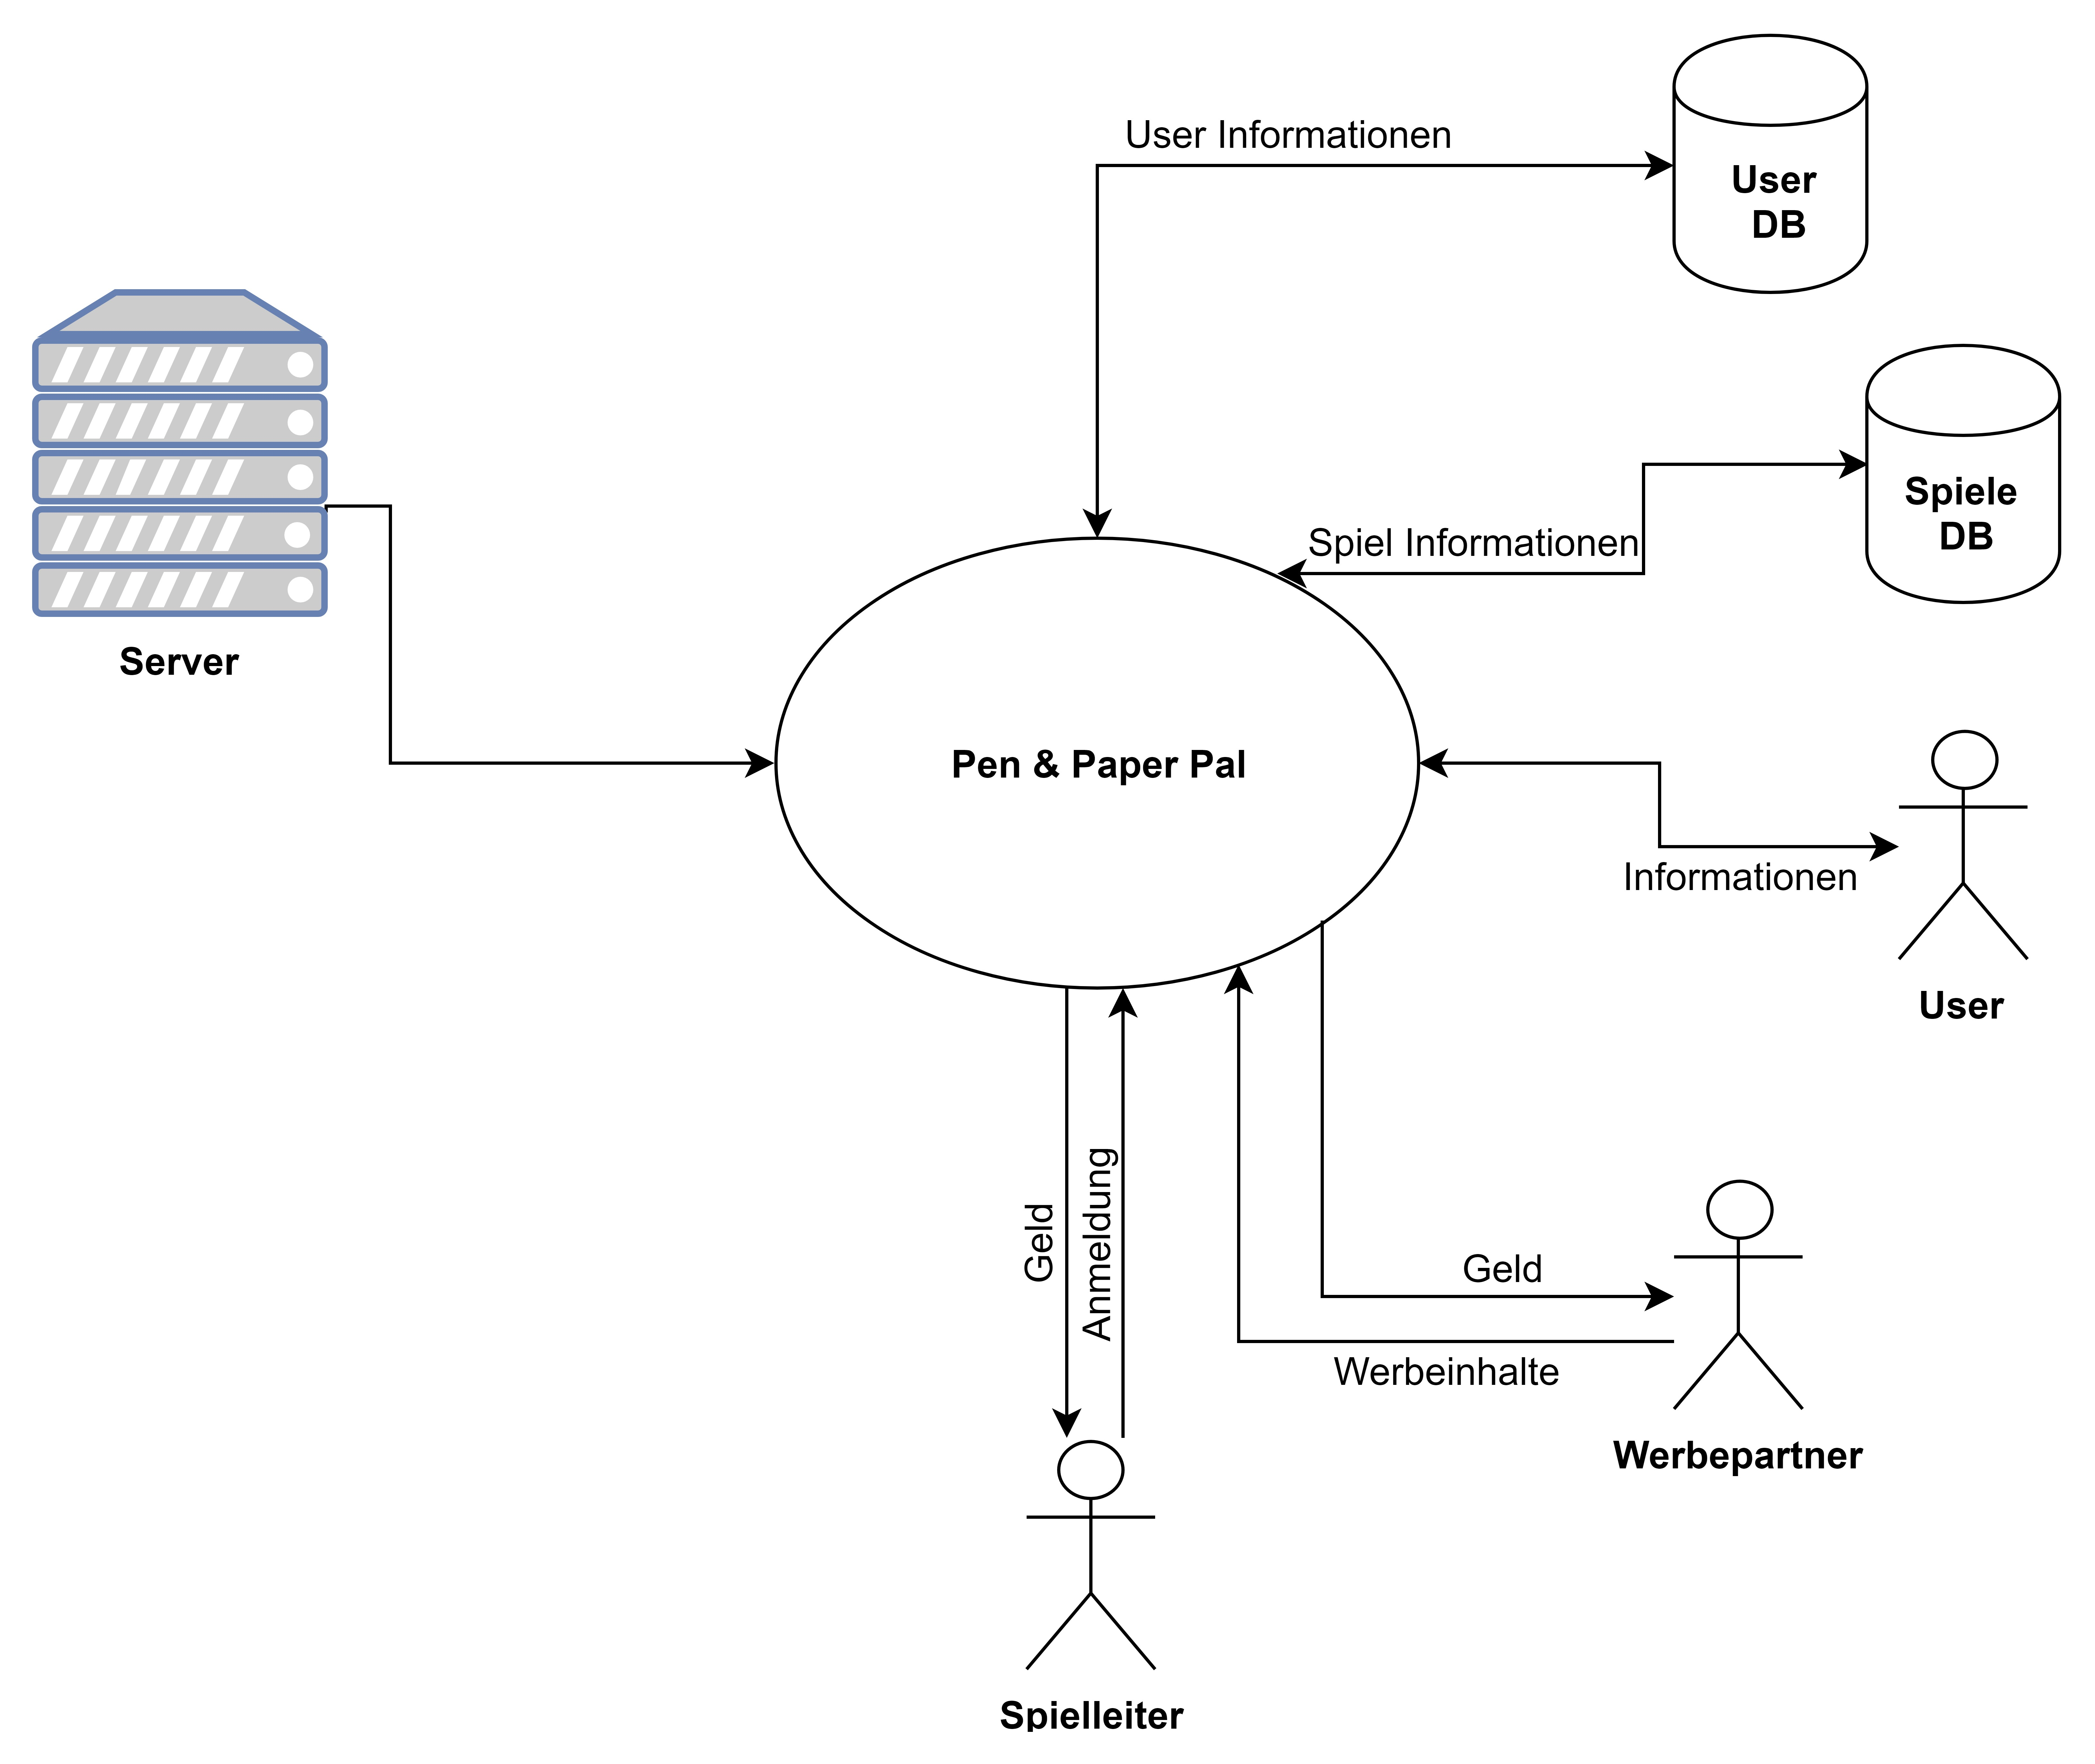
\includegraphics[width = \textwidth]{docs/03_03_Systemkontext.jpg}
\end{figure}

\section{Stakeholderanalyse}

\section{Requirementsengineering}
\begin{tabularx}{\textwidth}{|c|X|}
	\hline
	\multicolumn{2}{|l|}{\colorcell{{Functional Requirements}}}\\
	\hline
	\colorcelllight{REQ01} & Der Benutzer muss sich anmelden können.\\
	\hline
	\colorcelllight{REQ02} & Ein neuer Anwender ohne Account muss sich registrieren können.\\
	\hline
	\colorcelllight{REQ03} & Benutzer muss Orte, andere Nutzer und Spiele bewerten können.\\
	\hline
	\colorcelllight{REQ04} & Benutzer müssen sich zu Spielgruppen zusammenschließen können.\\
	\hline
	\colorcelllight{REQ05} & Benutzer müssen andere suchende Spieler (unter Angabe eines Ortes sowie eines Umkreises) finden können.\\
	\hline
	\colorcelllight{REQ06} & Benutzer sollen sich innerhalb der Gruppe unterhalten können.\\
	\hline
	\colorcelllight{REQ07} & Benutzer sollen untereinander kommunizieren können.\\
	\hline
	\colorcelllight{REQ08} & Benutzer soll per GPS suchende Spieler im Umkreis finden können.\\
	\hline
	\colorcelllight{REQ09} & Benutzer soll Suche filtern können.\\
	\hline
	\colorcelllight{REQ10} & Benutzer soll innerhalb der Gruppe einen gemeinsamen Termin finden können.\\
	\hline
	\colorcelllight{REQ11} & Benutzer sollen an einer Tauschbörse ihre Spiele tauschen können.\\
	\hline
	\colorcelllight{REQ12} & Benutzer sollen sich in einem Forum austauschen können.\\
	\hline
	\multicolumn{2}{|l|}{\colorcell{Non-Functional Requirements}}\\
	\hline
	\colorcelllight{REQ13} & Server muss immer erreichbar sein.\\
	\hline
	\colorcelllight{REQ14} & Server muss durchschnittlich innerhalb von 20ms antworten.\\
	\hline
	\colorcelllight{REQ15} & Miner muss immer minen.\\
	\hline
	\colorcelllight{REQ16} & Das Projekt soll nach Kanban geführt werden.\\
	\hline
	\multicolumn{2}{|l|}{\colorcell{Risiken}}\\
	\hline
	\colorcelllight{RSK01} & Größe des Projekts wurde überschätzt (Projekt \& Produkt).\\
	\hline
	\colorcelllight{RSK02} & Ein Konkurrenz-Produkt erreicht den Markt vor Systemfertigstellung.\\
	\hline
	\colorcelllight{RSK03} & Projekt erwirtschaftet zu wenig Geld.\\
	\hline
\end{tabularx}

\end{document}